\documentclass{beamer}

\mode<presentation>
{
  \usetheme{Antibes}
  \usecolortheme{beaver}
  % or ...

  \setbeamercovered{transparent}
  % or whatever (possibly just delete it)
}


\usepackage[english]{babel}
\usepackage[utf8]{inputenc}
\usepackage{times}
\usepackage[T1]{fontenc}
\usepackage{graphicx}
\usepackage[compatibility=false]{caption}
\usepackage{subcaption}
\usepackage{physics}
\usepackage{amsmath}
\usepackage{amssymb}

%\usepackage{multimedia}
%\usepackage{movie9}


\newcommand{\expv}[1]{\ensuremath{\mathbb{E}[ #1]}}
\newcommand{\xs}[2]{\ensuremath{\Sigma_{#1}^{(#2)}}}
\newcommand{\intO}{\ensuremath{\int\limits_{4\pi}}}
\newcommand{\intz}{\ensuremath{\int\limits_0^1}}
\newcommand{\intf}{\ensuremath{\int\limits_{-\infty}^\infty}}
\newcommand{\intzf}{\ensuremath{\int\limits_{0}^\infty}}

\title[Numerical UQ Methods] % (optional, use only with long paper titles)
{Numerical Methods\\ for\\ Uncertainty Quantification}

%\subtitle
%{A Term Project}

\author[Talbot] % (optional, use only with lots of authors)
{Paul W. Talbot\inst{1}}


\institute[University of New Mexico] % (optional, but mostly needed)
{
  \inst{1}%
  University of New Mexico\\
   \vspace{10pt}
\footnotesize{Supported by Idaho National Laboratory}
}

\date[BYU-I, 2014] % (optional, should be abbreviation of conference name)
{BYU-Idaho Physics Colloquium, February 26th 2015}


\subject{Uncertainty Quantification}

\pgfdeclareimage[height=0.5cm]{university-logo}{../graphics/unmlogo}
%\logo{\pgfuseimage{university-logo}}
\logo{\makebox[0.95\paperwidth]{
  
\includegraphics[height=1cm]{../graphics/INL}\hfill
    
\includegraphics[height=0.5cm]{../graphics/unmlogo}}

}

\addtobeamertemplate{navigation symbols}{}{
  \usebeamerfont{footline}%
  \usebeamercolor[fg]{footline}%
  \hspace{1em}%
  \insertframenumber/\inserttotalframenumber
}

\begin{document}

\begin{frame}
  \titlepage
\end{frame}

\begin{frame}{Outline}{Discussion Points}\vspace{-20pt}
  \tableofcontents[pausesections]
  % You might wish to add the option [pausesections]
\end{frame}

\section{Sources of Uncertainty}
\begin{frame}{Uncertainty}
\begin{itemize}
\item Aleatory (physical)
\begin{itemize}
  \item Quantum effects, 
\end{itemize}
\item Epistemic (measured)
\end{itemize}
\end{frame}

\begin{frame}{Example Stochastic Problem}\vspace{-30pt}
\begin{equation}
y_f=y_i + v\sin(\theta)t - \frac{1}{2}gt^2,
\end{equation}
\begin{equation}
x_f=v\cos(\theta)t.
\end{equation}
  \begin{figure}[h!]
    \centering
      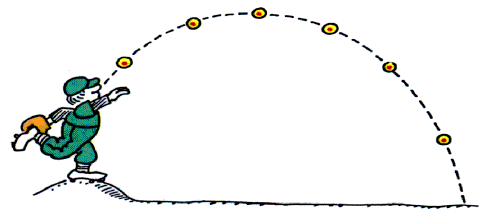
\includegraphics[width=0.5\textwidth]{../graphics/projectile}
  \end{figure}
\vspace{-10pt}
Solution: $x_f=\frac{v\cos{\theta}}{g}\left(v\sin\theta+\sqrt{v^2\sin^2\theta + 2gy_i}\right)$
\end{frame}

\begin{frame}{Example Stochastic Problem}\vspace{-50pt}

\begin{equation}
x_f=\frac{v\cos{\theta}}{g}\left(v\sin\theta+\sqrt{v^2\sin^2\theta + 2gy_i}\right)
\end{equation}
\begin{itemize}
\item initial height $y_i = 2$ m
\item initial velocity $v = 50$ m/s
\item initial trajectory $\theta = 35^o$
\item accel. gravity $g = -9.81$ m/s/s
\end{itemize}
\end{frame}

\begin{frame}{Example Stochastic Problem}\vspace{-50pt}
\begin{equation}
x_f=\frac{v\cos{\theta}}{g}\left(v\sin\theta+\sqrt{v^2\sin^2\theta + 2gy_i}\right)
\end{equation}
\begin{itemize}
\item initial height $y_i = 1\pm1$ m
\item initial velocity $v = 50\pm5$ m/s
\item initial trajectory $\theta = 45\pm10^o$
\item accel. gravity $g = 9.7988 \pm0.0349$ m/s/s
\end{itemize}
\end{frame}

\section{Analytic Methods}
\begin{frame}{Uncertainty Quantification}\vspace{-20pt}
\[x_f=\frac{v\cos{\theta}}{g}\left(v\sin\theta+\sqrt{v^2\sin^2\theta + 2gy_i}\right)\]
Min-Max
\tiny
\[x_{f,\text{min}}=\frac{(45)(0.5736)}{9.7369}\left((45)(0.8192)+\sqrt{(45)^2(0.8192)^2+2(9.7369)(0)}\right)= 195.45 \text{ m}\]
\[x_{f,\text{max}}=\frac{(55)(0.8192)}{9.8337}\left((55)(0.5736)+\sqrt{(55)^2(0.5736)^2+2(9.8337)(2)}\right)= 291.92 \text{ m}\]
\normalsize
Result: $x_f\approx244\pm48$ m \vspace{15pt}\\ \pause
Flawed Reasoning
\begin{itemize}
\item Nonlinear Flight Path
\item Does increasing $\theta$ make a longer or shorter range?
\end{itemize}
\end{frame}

\begin{frame}{Uncertainty Quantification}\vspace{-30pt}
$x_f=\frac{v\cos{\theta}}{g}\left(v\sin\theta+\sqrt{v^2\sin^2\theta + 2gy_i}\right)$\\\vspace{10pt}
Analytic Uncertainty
\[\sigma_{x_f} = \sqrt{\left(\pdv{x_f}{y_i}\right)^2\sigma_{y_i}^2 + \left(\pdv{x_f}{v}\right)^2\sigma_{v}^2 + \left(\pdv{x_f}{g}\right)^2\sigma_{g}^2 + \left(\pdv{x_f}{\theta}\right)^2\sigma_{\theta}^2}\]% \vspace{20pt}\\
Result: $x_f=256\pm51$ m  \vspace{10pt}\\
Works well for simple functions
\begin{itemize}
\item Simple derivatives
\item Analytic solution
\end{itemize}
\end{frame}

\begin{frame}{A More Difficult Problem}
%No Air Resistance:
%\begin{equation}
%y_f=v\sin(\theta)t - \frac{1}{2}gt^2,
%\end{equation}
%\begin{equation}
%x_f=v\cos(\theta)t.
%\end{equation}
\vspace{-20pt}With Air Resistance:
\begin{equation}
y_f=\frac{v_t}{g}(v\sin\theta+v_t)\left(1-e^{-gt/v_t}\right)-v_tt,
\end{equation}
\begin{equation}
x_f=\frac{vv_t\cos\theta}{g}\qty(1-e^{-gt/v_t}).
\end{equation}
\begin{equation}
v_t=\frac{mg}{D},\hspace{20pt}D=\frac{\rho C A}{2},\hspace{20pt}A=\pi r^2
\end{equation}
\hspace{30pt}Solve numerically to get $x_f$ (Forward Euler).
\end{frame}

\begin{frame}{A More Difficult Problem}
\vspace{-30pt}Forward Euler\\
\texttt{while $y_k>0$:}
\begin{align*}
a^{(x)}_{k+1} = \frac{-D}{m}v_k\ v_k^{(x)},&\hspace{15pt}a^{(y)}_{k+1} = -g-\frac{D}{m}v_k\ v_k^{(x)},\\[15pt]
v^{(x)}_{k+1} =v^{(x)}_{k}+ a^{(x)}_{k+1}\Delta_t,&\hspace{15pt}v^{(y)}_{k+1} =v^{(y)}_{k}+ a^{(y)}_{k+1}\Delta_t,\\[15pt]
x_{k+1} =x_k+ v_{k+1}^{(x)}\Delta_t + \frac{1}{2}a_{k+1}^{(x)} \Delta_t^2,&\hspace{15pt}y_{k+1} =y_k+ v_{k+1}^{(y)}\Delta_t + \frac{1}{2}a_{k+1}^{(y)} \Delta_t^2.
\end{align*}
(video)
\end{frame}

\begin{frame}{Additional Uncertainty}
\begin{equation}
y_f=\frac{v_t}{g}(v\sin\theta+v_t)\left(1-e^{-gt/v_t}\right)-v_tt,
\end{equation}
\begin{equation}
x_f=\frac{vv_t\cos\theta}{g}\qty(1-e^{-gt/v_t}).
\end{equation}
\begin{equation}
v_t=\frac{mg}{D},\hspace{20pt}D=\frac{\rho C A}{2},\hspace{20pt}A=\pi r^2
\end{equation}
\begin{align}
m=0.145\pm0.0725\text{ kg},\hspace{30pt}&r=0.0336\pm0.00336\text{ m},\\
C=0.5\pm0.5,\hspace{35pt}&\rho_\text{air}=1.2\pm0.1\text{ kg/m$^3$}.
\end{align}
\end{frame}

\section{Numerical Methods}
\begin{frame}{Uncertainty Quantification: Complicated Problems}\vspace{-20pt}
How do we quantify uncertainty for problems without simple analytic solutions?\vspace{15pt}
\begin{itemize}
\item Monte Carlo sampling
\item Stochastic Collocation
\item High Density Model Reduction (low-order)
\end{itemize}
\end{frame}

\begin{frame}{Uncertainty Quantification}{Monte Carlo}\vspace{-30pt}
\begin{itemize}
\item Let $u(Y)$ be any system, like $x_f(v,\theta,g,y_i$)
\item Randomly sample input parameters, record outputs
\item Repeat $M$ times
\item Calculate moments (mean, variance, skew, kurtosis)
\end{itemize}
\centerline{Mean: $\bar u\approx\frac{1}{M}\sum u\left(Y^{(m)}\right)$}
(video)
\end{frame}

\end{document}


